% !TEX TS-program = pdflatex
% !TEX encoding = UTF-8 Unicode

% This is a simple template for a LaTeX document using the "article" class.
% See "book", "report", "letter" for other types of document.

\documentclass[11pt]{article} % use larger type; default would be 10pt

\usepackage[utf8]{inputenc} % set input encoding (not needed with XeLaTeX)

%%% Examples of Article customizations
% These packages are optional, depending whether you want the features they provide.
% See the LaTeX Companion or other references for full information.

%%% PAGE DIMENSIONS
\usepackage{geometry} % to change the page dimensions
\geometry{a4paper} % or letterpaper (US) or a5paper or....
% \geometry{margin=2in} % for example, change the margins to 2 inches all round
% \geometry{landscape} % set up the page for landscape
%   read geometry.pdf for detailed page layout information

\usepackage{graphicx} % support the \includegraphics command and options

% \usepackage[parfill]{parskip} % Activate to begin paragraphs with an empty line rather than an indent

%%% PACKAGES
\usepackage{booktabs} % for much better looking tables
\usepackage{array} % for better arrays (eg matrices) in maths
\usepackage{paralist} % very flexible & customisable lists (eg. enumerate/itemize, etc.)
\usepackage{verbatim} % adds environment for commenting out blocks of text & for better verbatim
\usepackage{subfig} % make it possible to include more than one captioned figure/table in a single float
% These packages are all incorporated in the memoir class to one degree or another...

%%% HEADERS & FOOTERS
\usepackage{fancyhdr} % This should be set AFTER setting up the page geometry
\pagestyle{fancy} % options: empty , plain , fancy
\renewcommand{\headrulewidth}{0pt} % customise the layout...
\lhead{}\chead{}\rhead{}
\lfoot{}\cfoot{\thepage}\rfoot{}

%%% SECTION TITLE APPEARANCE
\usepackage{sectsty}
\allsectionsfont{\sffamily\mdseries\upshape} % (See the fntguide.pdf for font help)
% (This matches ConTeXt defaults)

%%% ToC (table of contents) APPEARANCE
\usepackage[nottoc,notlof,notlot]{tocbibind} % Put the bibliography in the ToC
\usepackage[titles,subfigure]{tocloft} % Alter the style of the Table of Contents
\renewcommand{\cftsecfont}{\rmfamily\mdseries\upshape}
\renewcommand{\cftsecpagefont}{\rmfamily\mdseries\upshape} % No bold!

%%% END Article customizations

%%% The "real" document content comes below...

\title{CSU34031 Advanced Telecommunications \\ Project II}
\author{Efeosa Eguavoen - 17324649}
%\date{} % Activate to display a given date or no date (if empty),
         % otherwise the current date is printed 

\begin{document}
\maketitle
\newpage
\section{Project Specificiation}
The aim of this project is to develop a secure social media application for Facebook, Twitter, WhatsApp etc., or for your own social networking app. For example, your application will secure the Facebook Wall, such that only people that are part of your “Secure Facebook Group” will be able to decrypt each other’s posts. To all other users of the system the post will appear as ciphertext. 
 You are required to design and implement a suitable key management system for your application that allows any member of the group to share social media messages securely, and allows you to add or remove people from a group. You are free to implement your application for a desktop or mobile platform and make use of any open source cryptographic libraries. 
 

\section{Overall Implementation}
To implement this project, I went with creating my own social media website using the Django framework for Python. I will split this report into 2 major sections:
\begin{itemize}
\item[1.] Views: The backend of the code and how things connect. A diagram of some description will be added also.
\item[2.] Models: Databases, Html code and other stuff used to implement the project.
\end{itemize}

\section{Views}
The project was made using Django, a web framework for Python that has a lot of built in features that makes it easier to get a website built and running quickly. The project is composed of 2 main applications: 
\begin{itemize}
\item[1.]Accounts : An app that manages user creation, login and user authentication. Also manages user profiles.
\item[2.]SecureApp: An app that manages user posts, creating connections between users and encryption.
\end{itemize}
\subsection{Accounts}
The accounts app is responsible for creating users for the social media application and logging them in. It also handles user account verification and their user profiles. On launch of the project, we first have to either login or register. Logging in is handled by Django using their authentication library that handles users and passwords securely by encrypting them and storing them in the system. The login form I've created verifies input and makes sure that nothing that shouldn't be entered is entered.Different error messages are returned depending on the type of error the user makes as defined in the forms.py file in accounts.
\begin{center}
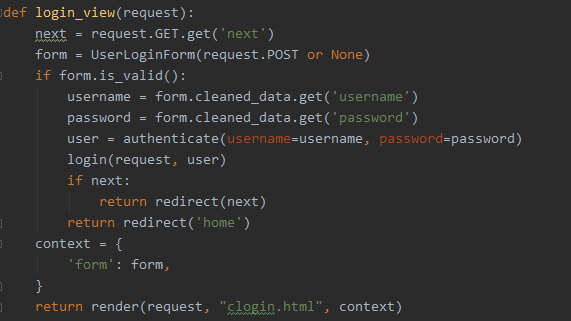
\includegraphics{login.png}
\end{center}

Account registration is handled in another function that asks the user for multiple pieces of data to register a new user to the system. Passwords are required to be of certain length and containing certain characters for security. Passwords are also asked to be entered twice for added security and to make sure the user isn't creating spam accounts. Different error messages are returned depending on the type of error the user makes as defined in the forms.py file in accounts.
\begin{center}
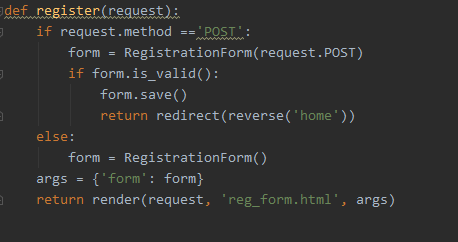
\includegraphics{register.png}
\end{center}

Account profiles are handled in this app also. Depending on wheter you're viewing your own profile or another profile, different things happen. If you're viewing your own profile, all you details and posts come up unencrypted as it's your own data you're looking at.
\newline
But if you're looking at another users profile, the system first checks if you're friends with the person. If you are, you can see their details and all their posts unencrypted. Also no option to add them as a friend is put up but an option to remove them as a friend is disaplayed. 
\newline
If you are not friends, all their posts are encrypted using the cryptography library in python. A key is generated and using this key, every post by that user is encrypted and cipher text is instead returned. You then have the option to add them as a friend to unencrypt their posts. But their posts will not be unencrypted until they also add you as a friend.
\begin{center}
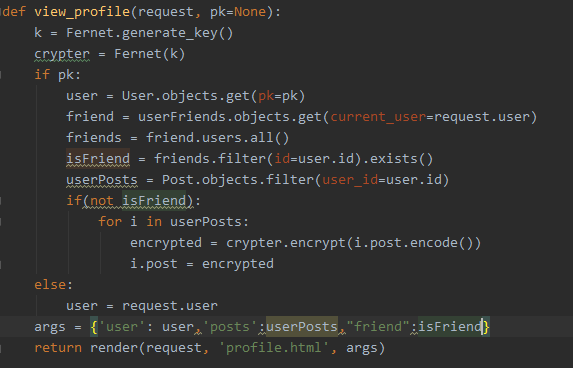
\includegraphics{view_profile.png}
\end{center}
\newpage
\subsection{SecureApp}
The actual social media aspect of the app sends you to a homescreen once you've logged. Here you can see posts from everyone on the app. But only posts from people you're friends with and are also friends with you are decrypted. Everyone else's text is ciphertext. 
\newline
We have the option to submit posts to the site for other users of your group to read. Members who are not part of your group will only see ciphertext
\begin{center}
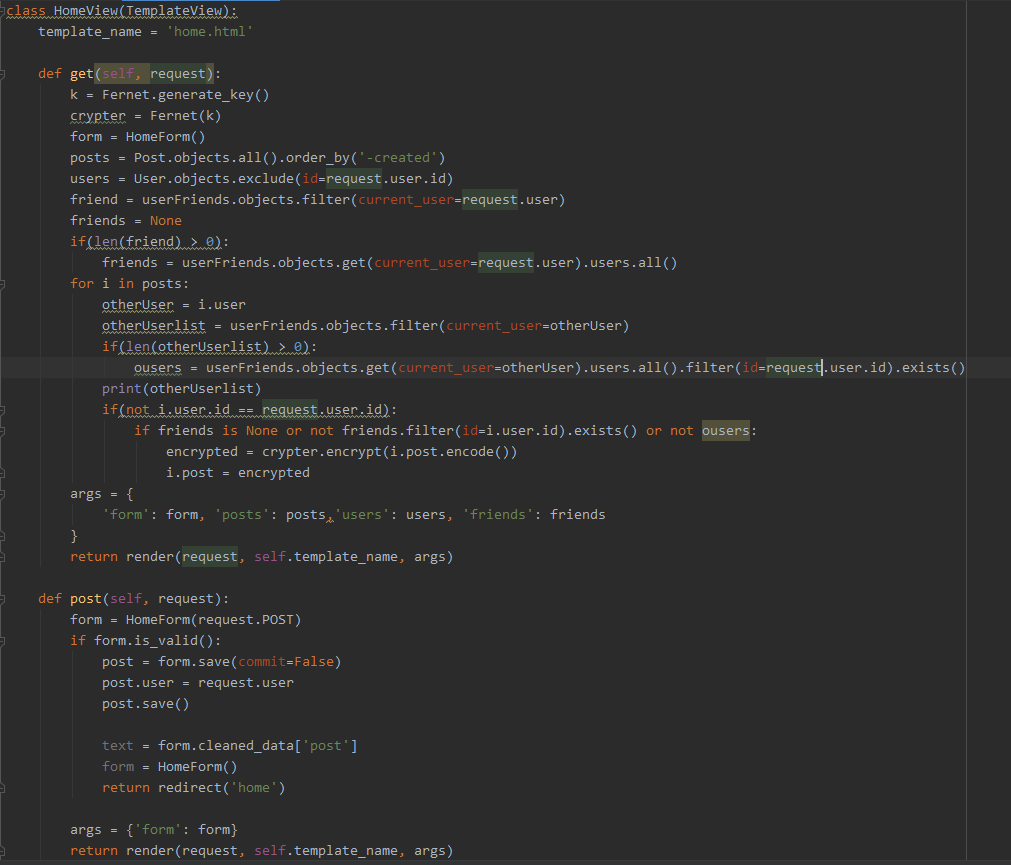
\includegraphics[scale = 0.6]{home.png}
\end{center}
Finally we can also add a friend, but as previously mentioned, their posts remain encrypted till they also add you as a friend.
You can also see all your friends on this page and have the option to remove friends if you wish. You can click on their names to look at their profiles if you wish
\begin{center}
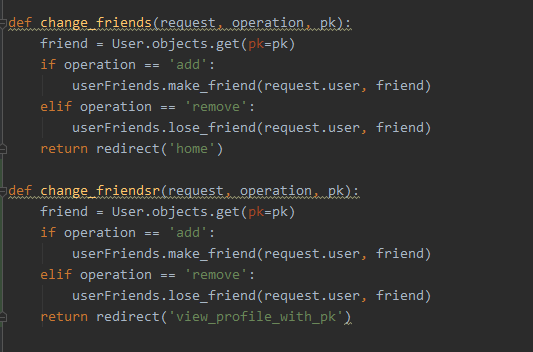
\includegraphics{frnds.png}
\end{center}

\subsection{Encryption}
For encryption in this app, I used the Cryptography library for python that's the default library used for encryption. The specific function used is called Fernet. It's an implementation of symmetric key authenticated cryptography. It uses AES with cipher block chaining as it's cryptographically strong as suitable for block ciphers. It creates a 128 bit key for encyption. For authentication, it uses HMAC, a cryptograohic hash function that's implemented using SHA 256 as it creates near unique signature for text.
\subsection{Diagram}
\begin{center}
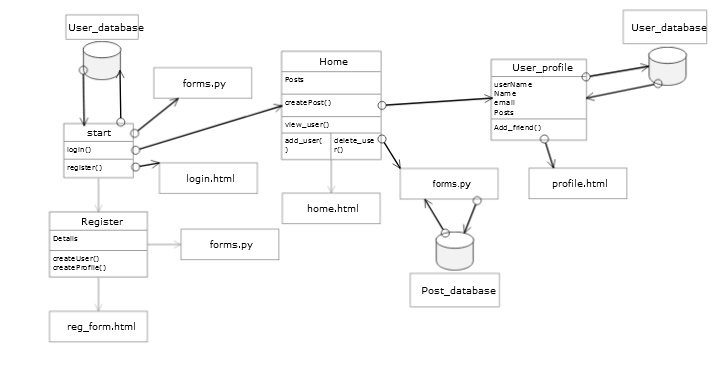
\includegraphics[scale = 0.9]{diagram.png}
\end{center}
\section{Models}
A number of other parts are necessary for the project to work. I used SQLite to manage users, posts and relationships between users. Forms were created to take in input from users and enter it into the application. Numerous HTML pages we're also created for the UI and such.
\section{Demo}
The demo can be located at the following Github link alongside the code: 
\newline
https://github.com/foesa/TweetSecure
\newline
In the attached Demo, I've shown a demonstration of the app working. You can see me create a new user and look at a post made by another user and it's encrypted. When I add the user it remains encrypted but they're added to my friends list. When I logout and login as the other user and add the user that requested, and then log back in as the other user, the post is then decrypted. If I remove the person from my group, their post becomes encrypted again. But once I add them back I can see their post as they didn't remove the current user as a friend. 
\newline
To run this yourself, clone the project and provided you have python installed, CD into TweetSecure/SocialMediaApp and then run manage.py. Otherwise, the attached Demo shows all functionality.
\end{document}
